% ==================================================================
% Chapter 4 — System Requirement Specification   (writer W4)
% ==================================================================
% Local TikZ styles used only by the UML diagrams of this chapter (prefixed srs).
\tikzset{
  srsactor/.pic={%
    \draw[thick] (0,0.62) circle (0.16);
    \draw[thick] (0,0.46)--(0,-0.02) (-0.28,0.28)--(0.28,0.28)
                 (0,-0.02)--(-0.22,-0.42) (0,-0.02)--(0.22,-0.42);},
  srscls/.style={draw,rectangle split,rectangle split parts=3,text width=3.25cm,
                 inner sep=2.5pt,font=\footnotesize,execute at begin node=\raggedright,
                 rectangle split part fill={black!7,white,white},
                 rectangle split part align={center,left,left}},
  srslife/.style={draw,fill=black!5,align=center,minimum height=0.95cm,text width=1.8cm,
                  font=\footnotesize,inner sep=2pt},
  srsmsg/.style={-{Stealth[length=2mm]}},
  srsret/.style={-{Stealth[length=2mm]},dashed},
  srsml/.style={above,font=\footnotesize,inner sep=1.5pt,fill=white},
  srsnote/.style={font=\footnotesize,align=left,inner sep=1.5pt,fill=white},
  srsframe/.style={draw,thin},
}

\chapter{System Requirement Specification}\label{ch:srs}

\section{Chapter overview}\label{sec:srs-overview}

\Cref{ch:method} explained how this research was conducted; this chapter specifies \emph{what} had to be built, bridging the stakeholder needs and objectives of \cref{sec:intro-objectives} and the implementation of \cref{ch:impl}. It identifies the stakeholders of the Pressure-based Real-time Intersection Signal Management (\prism{}) controller with an onion model (\cref{sec:srs-stakeholders}), and shows how the concerns of the Piliyandala Traffic Police and the Road Development Authority (RDA), together with the drone dataset fields, were operationalised into variables, objectives and requirements (\cref{sec:srs-operationalisation}). The system is then analysed with Unified Modelling Language (UML) use case, class, activity and sequence diagrams (\cref{sec:srs-usecase,sec:srs-class,sec:srs-activity,sec:srs-sequence}), followed by the layered architecture (\cref{sec:srs-arch}) and the prioritised requirements (\cref{sec:srs-requirements}) that later guided the test cases of \cref{ch:eval}.

The system has no web front-end: results were inspected through SUMO-GUI, the graphical interface of the Simulation of Urban MObility (\sumo{}) package, and through exported tables and plots. Artificial intelligence was used only for vehicle detection; the signal controller is pure mathematics.

% ------------------------------------------------------------------
\section{Stakeholder analysis}\label{sec:srs-stakeholders}

Stakeholders were identified with the onion model of Alexander~\cite{alexander2005taxonomy}, which arranges them in concentric layers by how directly they interact with the product. The innermost layer is the system itself: the Drone Trajectory eXtractor (\dtx{}), the Virtual LiDAR Sensor (\vls{}) and \prism{}. The \emph{containing system} holds those who operate it: the traffic engineer or researcher, and the traffic police who currently control the junction and would operate a deployed controller. The \emph{wider environment} contains those affected without operating it: commuters, motorcyclists and three-wheeler drivers, bus operators, pedestrians, the RDA as road owner, and the supervisor. An outer \emph{regulatory} layer was added because the drone survey required the Civil Aviation Authority of Sri Lanka (CAASL) and the Ministry of Defence (MoD)~\cite{caasl_drone}. \Cref{fig:srs-onion} shows the model and \cref{tab:srs-stakeholders} each stakeholder's role, viewpoint and influence.

\begin{figure}[htbp]
\centering
\resizebox{\textwidth}{!}{%
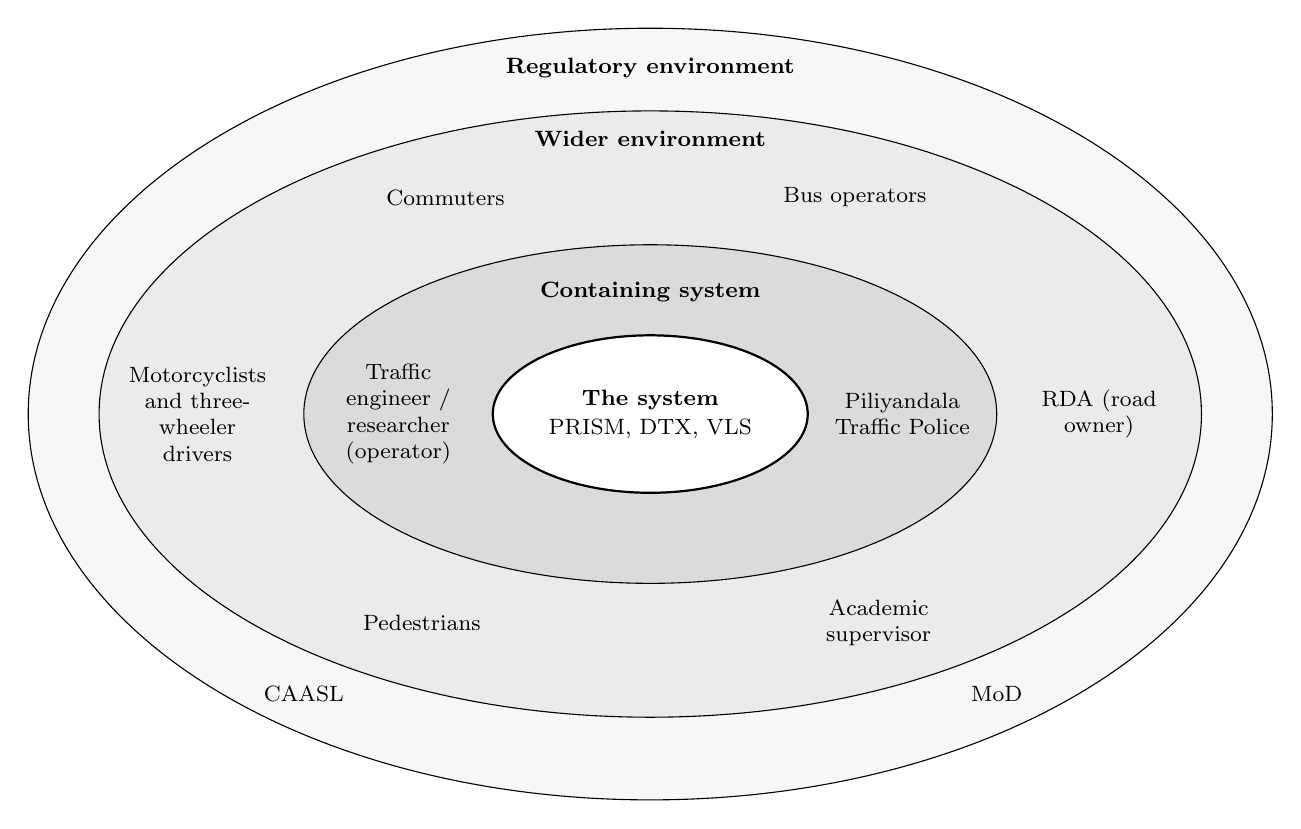
\begin{tikzpicture}[font=\footnotesize,sh/.style={align=center,inner sep=1pt}]
  \draw[fill=black!3]  (0,0) ellipse (7.9cm and 4.9cm);
  \draw[fill=black!8]  (0,0) ellipse (7.0cm and 3.85cm);
  \draw[fill=black!14] (0,0) ellipse (4.4cm and 2.15cm);
  \draw[fill=white,thick] (0,0) ellipse (2.0cm and 1.0cm);
  % layer titles
  \node[font=\footnotesize\bfseries] at (0,4.4) {Regulatory environment};
  \node[font=\footnotesize\bfseries] at (0,3.5) {Wider environment};
  \node[font=\footnotesize\bfseries] at (0,1.55) {Containing system};
  \node[sh,font=\footnotesize\bfseries] at (0,0) {The system\\[1pt]\normalfont PRISM, DTX, VLS};
  % containing system
  \node[sh,text width=2.0cm] at (-3.2,0) {Traffic engineer / researcher (operator)};
  \node[sh,text width=2.0cm] at (3.2,0) {Piliyandala Traffic Police};
  % wider environment
  \node[sh,text width=1.9cm] at (-5.75,0) {Motorcyclists and three-wheeler drivers};
  \node[sh,text width=1.7cm] at (5.7,0) {RDA (road owner)};
  \node[sh,text width=2.9cm] at (-2.6,2.75) {Commuters};
  \node[sh,text width=2.9cm] at (2.6,2.75) {Bus operators};
  \node[sh,text width=2.4cm] at (-2.9,-2.65) {Pedestrians};
  \node[sh,text width=2.4cm] at (2.9,-2.65) {Academic supervisor};
  % regulators
  \node[sh] at (-4.4,-3.55) {CAASL};
  \node[sh] at (4.4,-3.55) {MoD};
\end{tikzpicture}}
\caption{Onion model of the stakeholders of the proposed system}
\label{fig:srs-onion}
\end{figure}

\begin{table}[htbp]
\centering
\caption{Stakeholder roles, viewpoints and influence}
\label{tab:srs-stakeholders}
\small
\renewcommand{\arraystretch}{1.15}
\begin{tabularx}{\textwidth}{@{}>{\raggedright\arraybackslash}p{2.5cm}>{\raggedright\arraybackslash}p{1.75cm}>{\raggedright\arraybackslash}X>{\raggedright\arraybackslash}X>{\raggedright\arraybackslash}p{1.65cm}@{}}
\toprule
\textbf{Stakeholder} & \textbf{Layer} & \textbf{Role} & \textbf{Interest / viewpoint} & \textbf{Influence}\\
\midrule
Traffic engineer / researcher & Containing & Builds, configures and runs DTX, SUMO, VLS and PRISM & Valid, reproducible and explainable results & High\\
Piliyandala Traffic Police & Containing & Controls the junction; switches lights off and directs traffic manually at peaks & Less officer time spent on manual control; safe operation & High\\
Commuters & Wider & End users of the junction & Shorter waiting and travel times & Medium\\
Motorcyclists and three-wheeler drivers & Wider & Majority of the vehicle mix; filter to the stop line & Fair treatment despite small size; not ignored by sensing & Low\\
Bus operators & Wider & Run scheduled services along the bypass & Reliable crossing times; high-occupancy vehicles weighted by PCU & Low\\
Pedestrians & Wider & Cross the arms between signal phases & Adequate and safe crossing time (future push-button phase) & Low\\
RDA & Wider & Owns the road and signal infrastructure & Lower congestion; a low-cost, deployable upgrade path & High\\
Academic supervisor & Wider & Guides and assesses the research & Academic rigour and ethical conduct & High\\
CAASL & Regulatory & Approves drone operations (SLCAIS 053) & Safe, lawful flights below 400~ft & High\\
MoD & Regulatory & Grants security clearance for flights & National security; restricted flight window & High\\
\bottomrule
\end{tabularx}
\end{table}

The analysis exposed a tension that shaped the design. The police and the RDA wanted lower waiting for \emph{every} road user, whereas a vehicle-count controller would favour the approach with the most vehicles regardless of size. Because motorcycles and three-wheelers dominated the observed traffic while buses carry many passengers, demand was weighted in Passenger Car Units (PCU) and a starvation cap ensured that no approach was neglected. Pedestrian and emergency-vehicle features were placed out of scope as future work. Influence was rated by the ability to stop or redirect the project: the police, the RDA and the regulators could withhold permission, and the supervisor approved the objectives, whereas road users influenced the design only indirectly through the data recorded about them.

% ------------------------------------------------------------------
\section{Operationalisation process}\label{sec:srs-operationalisation}

\begin{sloppypar}
Operationalisation turns abstract concerns into measurable variables~\cite{hudaib2018requirements}. Two primary sources were used: the discussion with the Piliyandala Traffic Police and the RDA on 17.09.2026, which produced two explicit needs and one explicit exclusion, and the trajectory dataset from the drone sessions of 02.10.2026, from whose fields every Key Performance Indicator (KPI) was computed. The literature gap of \cref{sec:lit-reflection} was a secondary source. \Cref{tab:srs-operationalisation} traces each item to a variable, to objectives O1--O7 and to the functional (FR) and non-functional (NFR) requirements of \cref{sec:srs-requirements}.
\end{sloppypar}

\begin{table}[htbp]
\centering
\caption[Operationalisation of stakeholder needs and dataset fields]{Operationalisation of stakeholder needs and dataset fields into variables, objectives and requirements}
\label{tab:srs-operationalisation}
\small
\renewcommand{\arraystretch}{1.15}
\begin{tabularx}{\textwidth}{@{}>{\raggedright\arraybackslash}p{3.0cm}>{\raggedright\arraybackslash}X>{\raggedright\arraybackslash}p{1.95cm}>{\raggedright\arraybackslash}p{2.4cm}@{}}
\toprule
\textbf{Source item} & \textbf{Measurable variable / KPI} & \textbf{Objective} & \textbf{Requirements}\\
\midrule
\multicolumn{4}{@{}l}{\textit{(a) Police / RDA discussion, 17.09.2026}}\\
Reduce officer time spent on manual traffic control & Share of cycles in which any approach queue exceeds 200~m (``manual-control trigger''); maximum queue length & O1, O6, O7 & FR10, FR12, FR14, FR16\\
Reduce waiting time for every road user & Mean waiting time per vehicle; 95th-percentile waiting time; waiting time per vehicle class & O1, O6, O7 & FR10, FR11, FR16, FR17\\
Emergency vehicles currently ``make way''; no priority logic requested & None in this study; recorded as future work & O1 & FR19 (W)\\
\midrule
\multicolumn{4}{@{}l}{\textit{(b) Drone trajectory dataset fields}}\\
Timestamp & Sample interval $\Delta t$; time in frame; flow per 5-min bin & O3, O4 & FR01, FR05, FR06\\
Vehicle class & Composition (\%); PCU flow; class-specific waiting & O3, O4, O6 & FR02, FR06, FR10\\
Position (pixel $\rightarrow$ metre) & Trajectory; queue length; distance to stop line & O3, O4 & FR03, FR04\\
Speed & Free-flow speed; discharge headways giving saturation flow & O3, O4 & FR05, FR06\\
Zone (approach / exit) & Turning movement; turning ratios; per-approach demand & O3, O4 & FR06, FR07\\
Waiting flag ($v<0.1$~m/s) & Per-vehicle waiting time $W_i$; observed mean waiting used as calibration target & O3, O4, O7 & FR05, FR16\\
\midrule
\multicolumn{4}{@{}l}{\textit{(c) Literature gap}}\\
Heterogeneous traffic, imperfect sensing, explainability & PCU-weighted pressure; sensor-noise cost (PRISM vs PRISM-GT); decision log & O2, O5, O6 & FR08, FR09, FR15, NFR03, NFR04\\
\bottomrule
\end{tabularx}
\end{table}

The first need, less manual control by officers, cannot be observed directly because officer behaviour was not simulated. Since officers intervene when queues grow so long that the fixed plan visibly fails, the share of cycles in which any approach queue exceeded 200~m was adopted as a ``manual-control trigger''. The second need was operationalised as mean waiting time per vehicle, complemented by the 95th-percentile and per-class waiting so that ``every road user'' was not averaged away.

Validity was justified in two ways. \emph{Construct validity} was supported by defining waiting identically on both sides of the comparison: \dtx{} counted a vehicle as waiting below 0.1~m/s inside an approach zone, the same threshold \sumo{} uses~\cite{lopez2018sumo}, so observed waiting was a legitimate calibration target. \emph{Triangulation} came from drawing requirements from three independent sources: practitioners, drone measurements and literature. FR10 (pressure-based phase selection) appears in all three, whereas FR19 (emergency pre-emption) rested on one remark and was deprioritised. The dataset itself was validated by the accuracy tests of \cref{sec:eval-dtx}, and the calibrated model was checked against observed counts and waiting times before any controller was compared, so that the requirements rested on measured rather than assumed traffic.

% ------------------------------------------------------------------
\section{System and model analysis}\label{sec:srs-analysis}

\subsection{Use case diagram}\label{sec:srs-usecase}

\Cref{fig:srs-usecase} presents the use case diagram. The \emph{traffic engineer or researcher} extracts trajectories, calibrates the model, configures scenarios, runs experiments and exports KPIs. The \emph{traffic police} observe the junction in SUMO-GUI; manual override is dashed because it is future work. Two system actors were modelled: \sumo{} supplies vehicle states and receives signal states through the Traffic Control Interface (TraCI)~\cite{wegener2008traci}, and the Virtual LiDAR is the only information source for \emph{Scan junction}. Every experiment includes the phase decision, every decision includes a scan, and the fail-safe extends the decision when the sensor stops returning objects.

\begin{figure}[htbp]
\centering
\resizebox{\textwidth}{!}{%
\begin{tikzpicture}[font=\footnotesize,
  uc/.style={ellipse,draw,minimum width=3.3cm,minimum height=0.85cm,align=center,inner sep=1pt},
  sysact/.style={draw,rectangle,align=center,minimum width=2.3cm,minimum height=1.0cm,fill=black!5},
  incl/.style={-{Stealth[length=2mm]},dashed},
  rl/.style={font=\footnotesize\itshape,fill=white,inner sep=1pt}]
  \draw[rounded corners] (2.6,-0.45) rectangle (11.4,9.45);
  \node[anchor=north] at (7,9.4) {\textbf{PRISM research platform}};
  % left column
  \node[uc] (u1) at (4.6,8.2) {UC01 Extract\\trajectories};
  \node[uc] (u2) at (4.6,7.0) {UC02 Calibrate\\model};
  \node[uc] (u3) at (4.6,5.8) {UC03 Configure\\scenario};
  \node[uc] (u4) at (4.6,4.6) {UC04 Run\\experiment};
  \node[uc] (u6) at (4.6,3.4) {UC06 Export\\KPIs};
  \node[uc] (u5) at (4.6,1.9) {UC05 Observe in\\SUMO-GUI};
  \node[uc,dashed] (u10) at (4.6,0.45) {UC10 Override\\manually (future)};
  % right column
  \node[uc] (u7) at (9.3,7.0) {UC07 Scan\\junction};
  \node[uc] (u8) at (9.3,4.6) {UC08 Decide\\phase};
  \node[uc] (u9) at (9.3,2.3) {UC09 Apply\\fail-safe};
  % human actors
  \pic at (0.6,6.0) {srsactor};
  \node[align=center,text width=1.7cm] at (0.6,5.05) {Traffic Engineer / Researcher};
  \pic at (0.6,1.35) {srsactor};
  \node[align=center,text width=1.7cm] at (0.6,0.55) {Traffic Police};
  \foreach \u in {u1,u2,u3,u4,u6} \draw (0.95,6.25) -- (\u.west);
  \draw (0.95,1.6) -- (u5.west);
  \draw[dashed] (0.95,1.6) -- (u10.west);
  % system actors
  \node[sysact] (vl) at (13.4,8.0) {\guillemotleft system\guillemotright\\Virtual LiDAR};
  \node[sysact] (su) at (13.4,4.6) {\guillemotleft system\guillemotright\\SUMO};
  \draw (vl.west) -- (u7.east);
  \draw (su.north west) -- (u7.south east);
  \draw (su.west) -- (u8.east);
  \draw (su.south west) -- (u9.east);
  % relationships
  \draw[incl] (u4.east) -- node[rl,above=1pt] {\guillemotleft include\guillemotright} (u8.west);
  \draw[incl] (u8.north) -- node[rl] {\guillemotleft include\guillemotright} (u7.south);
  \draw[incl] (u9.north) -- node[rl] {\guillemotleft extend\guillemotright} (u8.south);
\end{tikzpicture}}
\caption{Use case diagram of the PRISM research platform}
\label{fig:srs-usecase}
\end{figure}

The three most important use cases are specified in \cref{tab:srs-uc-run,tab:srs-uc-decide,tab:srs-uc-extract}; the others are simple configuration or viewing actions.

\begin{table}[htbp]
\centering
\caption{Use case specification: UC04 Run experiment}
\label{tab:srs-uc-run}
\small
\renewcommand{\arraystretch}{1.15}
\begin{tabularx}{\textwidth}{@{}>{\raggedright\arraybackslash}p{2.8cm}>{\raggedright\arraybackslash}X@{}}
\toprule
\textbf{Field} & \textbf{Description}\\
\midrule
ID and name & UC04 -- Run experiment\\
Actors & Traffic engineer / researcher (primary); SUMO (system)\\
Description & Executes every combination of scenario, controller and seed and stores the KPIs of each run.\\
Pre-conditions & Network, route and vehicle-type files exist; \texttt{scenarios.yaml} lists scenarios, controllers (B1, B2, B3, PRISM, PRISM-GT) and seeds 6--15.\\
Main flow & 1.~Researcher starts the runner with the configuration file.\newline
2.~For each scenario, controller and seed the runner starts SUMO with the seed.\newline
3.~The simulation is stepped for 300~s of warm-up and 3,600~s of measurement; UC08 is included every 1~s.\newline
4.~SUMO trip, queue and emission outputs are parsed into a KPI row.\newline
5.~After all runs, statistics and plots are produced (FR17).\\
Alternative flow & 2a.~SUMO fails to start or a run aborts: the error is logged, the run is marked failed and the runner continues with the next combination.\\
Post-conditions & One KPI Comma-Separated Values (CSV) file per run, a summary table and plots exist; configuration and seeds are stored with the results.\\
\bottomrule
\end{tabularx}
\end{table}

\begin{table}[htbp]
\centering
\caption{Use case specification: UC08 Decide phase (control step)}
\label{tab:srs-uc-decide}
\small
\renewcommand{\arraystretch}{1.15}
\begin{tabularx}{\textwidth}{@{}>{\raggedright\arraybackslash}p{2.8cm}>{\raggedright\arraybackslash}X@{}}
\toprule
\textbf{Field} & \textbf{Description}\\
\midrule
ID and name & UC08 -- Decide phase (control step)\\
Actors & SUMO and Virtual LiDAR (system actors); initiated by UC04\\
Description & Every 1~s the controller decides whether to extend the current green or to terminate it, and which phase follows.\\
Pre-conditions & A phase is green; minimum and maximum greens, intergreen and starvation cap are configured.\\
Main flow & 1.~UC07 returns the tracked object list.\newline
2.~PRISM computes movement pressures, phase scores and the required green.\newline
3.~The rules of \cref{sec:srs-activity} are evaluated in order; the result is ``extend'' or ``terminate''.\newline
4.~On termination, 3~s amber and 2~s all-red are applied and the next phase is selected.\newline
5.~The signal state string is sent to SUMO and the decision and its reason are logged.\\
Alternative flow & 1a.~Five consecutive empty scans: UC09 applies the observed 78~s fixed-time plan until objects reappear.\newline
3a.~An exit link is above 85\% occupancy: phases feeding it are limited to their minimum green.\\
Post-conditions & No conflicting greens were issued; the decision record holds the scores and the rule that fired.\\
\bottomrule
\end{tabularx}
\end{table}

\begin{table}[htbp]
\centering
\caption{Use case specification: UC01 Extract trajectories}
\label{tab:srs-uc-extract}
\small
\renewcommand{\arraystretch}{1.15}
\begin{tabularx}{\textwidth}{@{}>{\raggedright\arraybackslash}p{2.8cm}>{\raggedright\arraybackslash}X@{}}
\toprule
\textbf{Field} & \textbf{Description}\\
\midrule
ID and name & UC01 -- Extract trajectories\\
Actors & Traffic engineer / researcher\\
Description & Converts a nadir drone video into metric vehicle trajectories, observed KPIs and SUMO route files.\\
Pre-conditions & Video file available; zone polygons, stop lines and at least four ground control points are defined; detector weights are fine-tuned.\\
Main flow & 1.~Each frame is stabilised to a reference frame.\newline
2.~Vehicles of seven classes are detected with tiled inference.\newline
3.~Detections are linked into tracks with persistent identities.\newline
4.~Pixel tracks are mapped to metres, smoothed and assigned to zones.\newline
5.~Waiting time, delay, flows, turning ratios and saturation flow are computed.\newline
6.~Route files and the observed-KPI CSV are written.\\
Alternative flow & 1a.~Too few feature matches: the frame is skipped and logged.\newline
4a.~A track is cut by the start or end of the video: it is counted in flows but excluded from averages (censored).\\
Post-conditions & Anonymous trajectory file, observed-KPI CSV and \texttt{.rou.xml} files exist; no images are stored.\\
\bottomrule
\end{tabularx}
\end{table}

\subsection{Class diagram}\label{sec:srs-class}

\begin{sloppypar}
\Cref{fig:srs-class} shows the static structure in three groups matching the artefacts. The extraction group is a pipeline from \texttt{Stabiliser} to \texttt{SumoExporter}, whose route files parameterise a \texttt{Scenario}. In the sensing group, \texttt{VirtualLidar} produces a noisy point list and \texttt{PerceptionTracker} aggregates confirmed \texttt{DetectedObject} instances. The control group centres on a \texttt{SignalController} interface with one \texttt{decide} operation: \texttt{PrismController} realises it and is composed of four \texttt{PhaseDefinition} objects and one \texttt{MovementState} per movement, while the abstract \texttt{BaselineController} is specialised into fixed-time, actuated and Webster controllers. Because \texttt{ExperimentRunner} depends only on the interface, all five controllers ran through the same code path, removing a common source of comparison bias. PRISM-GT is the same \texttt{PrismController} fed noise-free objects.
\end{sloppypar}

\begin{figure}[p]
\centering
\resizebox{\textwidth}{!}{%
\begin{tikzpicture}[font=\footnotesize,
  as/.style={-{Stealth[length=2mm]}},
  gen/.style={-{Triangle[open,length=2.6mm,width=2.6mm]}},
  real/.style={dashed,-{Triangle[open,length=2.6mm,width=2.6mm]}},
  comp/.style={{Diamond[length=3mm,width=2mm]}-},
  agg/.style={{Diamond[open,length=3mm,width=2mm]}-},
  ml/.style={font=\footnotesize,inner sep=1pt}]
  \def\cA{0}\def\cB{4.1}\def\cC{8.2}\def\cD{12.3}
  % ---------------- extraction (DTX)
  \node[srscls,anchor=north] (stab) at (\cA,0) {\centering \textbf{Stabiliser}\par\nodepart{second}refFrame: Image\\matcher: ORB+RANSAC\nodepart{third}stabilise(frame)};
  \node[srscls,anchor=north] (det) at (\cB,0) {\centering \textbf{Detector}\par\nodepart{second}model: YOLOv8s\\tiles: 2$\times$2, overlap 0.2\nodepart{third}detect(frame)};
  \node[srscls,anchor=north] (trk) at (\cC,0) {\centering \textbf{Tracker}\par\nodepart{second}trackThresh: 0.5\\matchThresh: 0.8\\buffer: 30\nodepart{third}update(detections)};
  \node[srscls,anchor=north] (geo) at (\cD,0) {\centering \textbf{Georeferencer}\par\nodepart{second}H: 3$\times$3 homography\\gsd: float\nodepart{third}toGround(px)};
  \node[srscls,anchor=north] (traj) at (\cD,-3.4) {\centering \textbf{TrajectoryBuilder}\par\nodepart{second}window: 11; order: 2\\zones: Polygon[ ]\nodepart{third}build(tracks)};
  \node[srscls,anchor=north] (met) at (\cC,-3.4) {\centering \textbf{MetricsCalculator}\par\nodepart{second}vStop: 0.1 m/s\\bin: 300 s\nodepart{third}waitingTime(traj)\\flows(); satFlow()};
  \node[srscls,anchor=north] (exp) at (\cB,-3.4) {\centering \textbf{SumoExporter}\par\nodepart{second}vTypes: dict\nodepart{third}writeRoutes(path)\\writeKpiCsv(path)};
  \node[font=\footnotesize\itshape,align=left,anchor=north west] at (-1.65,-3.45) {Extraction\\pipeline\\(DTX)};
  % ---------------- sensing + scenario
  \node[srscls,anchor=north] (scn) at (\cA,-7.0) {\centering \textbf{Scenario}\par\nodepart{second}name; routeFile\\demandLevel\nodepart{third}load()};
  \node[srscls,anchor=north] (vl) at (\cB,-7.0) {\centering \textbf{VirtualLidar}\par\nodepart{second}R: 75 m; height: 6 m\\$\sigma_0$: 0.10 m; $\lambda$: 0.2\nodepart{third}scan(t)};
  \node[srscls,anchor=north] (pt) at (\cC,-7.0) {\centering \textbf{PerceptionTracker}\par\nodepart{second}gate: 2.5 m\\$\alpha$: 0.5; $\beta$: 0.1\nodepart{third}update(scan)\\mapMatch(obj)};
  \node[srscls,anchor=north] (obj) at (\cD,-7.0) {\centering \textbf{DetectedObject}\par\nodepart{second}x, y, v, heading\\sizeClass; pcu\\approach; lane; dStop\nodepart{third}eta()};
  % ---------------- control + experiments
  \node[srscls,anchor=north] (run) at (\cA,-10.9) {\centering \textbf{ExperimentRunner}\par\nodepart{second}scenarios; seeds\\controllers\nodepart{third}run()\\collectKpis()};
  \node[srscls,anchor=north] (sc) at (\cB,-10.9) {\centering \guillemotleft interface\guillemotright\\\textbf{SignalController}\par\nodepart{second}--\nodepart{third}decide(objects, t)\\reset()};
  \node[srscls,anchor=north] (pr) at (\cC,-10.9) {\centering \textbf{PrismController}\par\nodepart{second}$\gamma,\delta,\kappa,\theta,\varepsilon,\rho$\\$G_{\min}$, $G_{\max}$, $T_{\mathrm{starve}}$\nodepart{third}pressure(m)\\score($\phi$); decide()};
  \node[srscls,anchor=north] (ph) at (\cD,-10.9) {\centering \textbf{PhaseDefinition}\par\nodepart{second}id: $\phi_1$..$\phi_4$\\movements; state\nodepart{third}greenState()};
  \node[srscls,anchor=north] (ms) at (\cC,-14.6) {\centering \textbf{MovementState}\par\nodepart{second}$Q_m$, $A_m$, $O_b$\\$R_\phi$; maxWait\nodepart{third}update(objects)};
  \node[srscls,anchor=north] (bl) at (\cB,-14.6) {\centering \guillemotleft abstract\guillemotright\\\textbf{BaselineController}\par\nodepart{second}plan\nodepart{third}decide(objects, t)};
  \node[srscls,anchor=north] (ft) at (\cA,-18.0) {\centering \textbf{FixedTimeController}\par\nodepart{second}cycle: 78 s\nodepart{third}decide()};
  \node[srscls,anchor=north] (ac) at (\cB,-18.0) {\centering \textbf{ActuatedController}\par\nodepart{second}minDur; maxDur\nodepart{third}decide()};
  \node[srscls,anchor=north] (wb) at (\cC,-18.0) {\centering \textbf{WebsterController}\par\nodepart{second}$C_0$; splits\nodepart{third}compute(Y, L)};
  % ---------------- associations
  \draw[as] (stab.east) -- (det.west);
  \draw[as] (det.east) -- (trk.west);
  \draw[as] (trk.east) -- (geo.west);
  \draw[as] (geo.south) -- (traj.north);
  \draw[as] (traj.west) -- (met.east);
  \draw[as] (met.west) -- (exp.east);
  \draw[as] (exp.west) -| node[ml,right,pos=0.75] {route files} (scn.north);
  \draw[as] (run.north east) -- node[ml,right,pos=0.4] {uses} (vl.south west);
  \draw[as] (vl.east) -- (pt.west);
  \draw[agg] (pt.east) -- node[ml,above,pos=0.6] {0..*} (obj.west);
  \draw[agg] (run.north) -- node[ml,right] {1..*} (scn.south);
  \draw[as] (run.east) -- (sc.west);
  \draw[real] (pr.west) -- (sc.east);
  \draw[gen] (bl.north) -- (sc.south);
  \draw[comp] (pr.east) -- node[ml,above,pos=0.6] {4} (ph.west);
  \draw[comp] (pr.south) -- node[ml,right] {1..*} (ms.north);
  \draw[as] (pr.north) -- node[ml,right] {reads} (pt.south);
  \draw[gen] (ft.north) |- ($(bl.south)+(0,-0.55)$) -- (bl.south);
  \draw (ac.north) -- ($(bl.south)+(0,-0.55)$);
  \draw (wb.north) |- ($(bl.south)+(0,-0.55)$);
\end{tikzpicture}}
\caption[Class diagram of the system components]{Class diagram of the extraction, sensing, control and experiment components}
\label{fig:srs-class}
\end{figure}

\subsection{Activity diagram}\label{sec:srs-activity}

\Cref{fig:srs-activity} formalises the decision loop implemented in \cref{sec:impl-prism}, run every $\Delta=1$~s. After five consecutive empty scans the controller assumes sensor failure and falls back to the observed 78~s fixed-time plan. Otherwise it updates the movement states and evaluates six ordered rules. A green never ends before its minimum (10~s through, 5~s right turn) and always ends at its maximum (50~s and 25~s). The fairness override ends it when another phase has waited $T_{\mathrm{starve}}=120$~s, and the spillback guard ends it after the minimum when an exit it feeds is over 85\% occupied. Gap-out ends a green serving nobody, and the pressure switch ends it when another phase's score exceeds the current one by a hysteresis margin after a fraction $\rho$ of the required green. Safety and fairness rules precede efficiency rules, so they can never be overridden. This ordering also bounds the worst-case red time of any phase by $T_{\mathrm{starve}}+G_{\max}+5$~s, and because every termination is attributable to exactly one rule, each decision can be logged with its reason, which satisfies the explainability requirement NFR04. Termination always inserts 3~s amber and 2~s all-red; the next phase is the oldest starved phase, otherwise the highest score.

\begin{figure}[p]
\centering
\begin{tikzpicture}[font=\footnotesize,node distance=0.42cm,
  act/.style={draw,rounded corners=4pt,align=center,text width=3.7cm,minimum height=0.75cm,inner sep=2pt},
  dec/.style={draw,diamond,aspect=2.6,align=center,text width=2.9cm,inner sep=0pt},
  fl/.style={-{Stealth[length=2mm]}},
  yl/.style={font=\footnotesize,inner sep=1pt}]
  \node[circle,fill=black,minimum size=0.35cm] (st) at (0,0) {};
  \node[act,below=0.4cm of st] (a1) {Start green of phase $g$;\\$t_g\leftarrow 0$};
  \node[act,below=of a1] (a2) {Wait $\Delta=1$~s; VLS scan and perception update};
  \node[dec,below=of a2] (d0) {$\geq 5$ consecutive empty scans?};
  \node[act,below=of d0] (a3) {Update $Q_m$, $A_m$, $O_b$, $R_\phi$; compute $S_\phi$ and $G_{\mathrm{req}}$};
  \node[dec,below=of a3] (d1) {$t_g<G_{\min}$?};
  \node[dec,below=of d1] (d2) {$t_g\geq G_{\max}$?};
  \node[dec,below=of d2] (d3) {Any $R_\phi\geq T_{\mathrm{starve}}$?};
  \node[dec,below=of d3] (d4) {Spillback: exit of $g$ with $O_b/C_b>0.85$?};
  \node[dec,below=of d4] (d5) {Gap-out: $\sum Q_g\leq 0.5$ PCU and no ETA $\leq 3$~s?};
  \node[dec,below=of d5] (d6) {$\max S_\phi>(1+\theta)S_g+\varepsilon$ and $t_g\geq\rho\,G_{\mathrm{req}}(g)$?};
  \node[act,below=of d6] (ext) {Extend green by 1~s};
  % right column
  \node[act,text width=3.2cm] (fs) at (7.0,0 |- d0) {Fail-safe: run observed 78~s fixed-time plan};
  \node[act,text width=3.2cm] (am) at (7.0,0 |- d2) {Terminate $g$:\\amber 3~s};
  \node[act,text width=3.2cm,below=of am] (ar) {All-red 2~s};
  \node[act,text width=3.2cm,below=of ar] (sel) {Next $g$: oldest starved phase, else $\arg\max S_\phi$ (ties $\phi_1\rightarrow\phi_4$)};
  % main flow
  \draw[fl] (st) -- (a1);
  \draw[fl] (a1) -- (a2);
  \draw[fl] (a2) -- (d0);
  \draw[fl] (d0) -- node[yl,right] {no} (a3);
  \draw[fl] (a3) -- (d1);
  \draw[fl] (d1) -- node[yl,right] {no} (d2);
  \draw[fl] (d2) -- node[yl,right] {no} (d3);
  \draw[fl] (d3) -- node[yl,right] {no} (d4);
  \draw[fl] (d4) -- node[yl,right] {no} (d5);
  \draw[fl] (d5) -- node[yl,right] {no} (d6);
  \draw[fl] (d6) -- node[yl,right] {no} (ext);
  % fail-safe
  \draw[fl] (d0.east) -- node[yl,above] {yes} (fs.west);
  \draw[fl] (fs.north) |- node[yl,above,pos=0.75] {next scan} (a2.east);
  % loops back to scan
  \draw[fl] (d1.west) -- node[yl,above] {yes} ++(-0.9,0) |- ($(a2.west)+(0,-0.12)$);
  \draw[fl] (ext.west) -- ++(-1.35,0) |- ($(a2.west)+(0,0.12)$);
  % terminate bus
  \coordinate (bus) at (4.25,0);
  \foreach \d in {d3,d4,d5,d6} \draw (\d.east) -- node[yl,above] {yes} (bus |- \d.east);
  \draw (bus |- d6.east) -- (bus |- d2.east);
  \draw[fl] (d2.east) -- node[yl,above,pos=0.3] {yes} (am.west);
  \draw[fl] (am) -- (ar);
  \draw[fl] (ar) -- (sel);
  \draw[fl] (sel.east) -- ++(0.35,0) |- (a1.east);
\end{tikzpicture}
\caption[Activity diagram of the PRISM decision loop]{Activity diagram of the PRISM decision loop, executed every 1~s of simulated time}
\label{fig:srs-activity}
\end{figure}

\subsection{Sequence diagrams}\label{sec:srs-sequence}

Three sequence diagrams, one per key use case, describe the run-time interactions. \Cref{fig:srs-seq-dtx} corresponds to UC01: each stabilised frame passes through YOLOv8~\cite{jocher2023yolov8} with Slicing Aided Hyper Inference (SAHI)~\cite{akyon2022sahi}, so that small motorcycles are found, and then ByteTrack~\cite{zhang2022bytetrack}. Georeferencing, smoothing and metrics follow the loop because smoothing and censoring need complete trajectories.

\begin{figure}[htbp]
\centering
\resizebox{\textwidth}{!}{%
\begin{tikzpicture}[font=\footnotesize]
  \def\ya{-0.3}\def\yb{-9.8}
  \foreach \x/\n/\t in {0/R/{\guillemotleft actor\guillemotright\\Researcher},2.25/S/Stabiliser,4.5/D/{Detector\\YOLOv8\\+ SAHI},6.75/T/{Tracker\\(ByteTrack)},9.0/G/{Geo-\\referencer},11.25/M/{Metrics\\Calculator},13.5/E/{Sumo\\Exporter}}{
    \node[srslife,text width=1.75cm] (\n) at (\x,0.3) {\t};
    \draw[dashed,black!60] (\x,\ya) -- (\x,\yb);}
  \draw[srsmsg] (0,-1.0) -- node[srsml] {run(video)} (2.25,-1.0);
  \draw[srsframe] (1.65,-1.4) rectangle (8.1,-6.2);
  \node[draw,fill=white,anchor=north west,inner sep=2pt] at (1.65,-1.4) {loop [each frame, 10~fps]};
  \draw[srsmsg] (2.25,-2.3) -- ++(0.4,0) -- ++(0,-0.45) -- (2.25,-2.75);
  \node[srsnote,anchor=west] at (2.7,-2.52) {warp (ORB\\+ RANSAC)};
  \draw[srsmsg] (2.25,-3.4) -- node[srsml] {detect(frame)} (4.5,-3.4);
  \draw[srsmsg] (4.5,-3.8) -- ++(0.4,0) -- ++(0,-0.45) -- (4.5,-4.25);
  \node[srsnote,anchor=west] at (4.95,-4.02) {2$\times$2 tiles\\+ merge};
  \draw[srsmsg] (4.5,-5.0) -- node[srsml] {detections} (6.75,-5.0);
  \draw[srsmsg] (6.75,-5.4) -- ++(0.4,0) -- ++(0,-0.45) -- (6.75,-5.85);
  \node[srsnote,anchor=west] at (7.2,-5.62) {assign\\IDs};
  \draw[srsmsg] (6.75,-6.8) -- node[srsml] {pixel tracks} (9.0,-6.8);
  \draw[srsmsg] (9.0,-7.4) -- node[srsml] {trajectories (m)} (11.25,-7.4);
  \draw[srsmsg] (11.25,-7.8) -- ++(0.4,0) -- ++(0,-0.45) -- (11.25,-8.25);
  \node[srsnote,anchor=west] at (11.7,-8.02) {$W_i$, flows,\\turns, $s$};
  \draw[srsmsg] (11.25,-8.8) -- node[srsml] {5-min flows} (13.5,-8.8);
  \draw[srsret] (13.5,-9.4) -- node[srsml] {\texttt{.rou.xml} and observed-KPI CSV} (0,-9.4);
\end{tikzpicture}}
\caption{Sequence diagram of the DTX extraction pipeline (UC01)}
\label{fig:srs-seq-dtx}
\end{figure}

\Cref{fig:srs-seq-control} shows one control step (UC08). The \texttt{VirtualLidar} reads ground truth from \sumo{}, but \texttt{PrismController} receives only the perception tracker's object list; its command returns to \sumo{} as a TraCI signal-state string. Keeping this boundary explicit in the design made it possible to swap the \vls{} for the noise-free oracle without touching the controller.

\begin{figure}[htbp]
\centering
\resizebox{\textwidth}{!}{%
\begin{tikzpicture}[font=\footnotesize]
  \def\ya{-0.3}\def\yb{-9.85}
  \foreach \x/\n/\t in {0/R/{Experiment\\Runner},3.8/S/{SUMO\\(TraCI)},7.0/V/{Virtual\\LiDAR},10.2/P/{Perception\\Tracker},13.4/C/{PRISM\\Controller}}{
    \node[srslife] (\n) at (\x,0.2) {\t};
    \draw[dashed,black!60] (\x,\ya) -- (\x,\yb);}
  \draw[srsframe] (-0.9,-0.8) rectangle (14.3,-9.6);
  \node[draw,fill=white,anchor=north west,inner sep=2pt] at (-0.9,-0.8) {loop [every 1~s of simulated time]};
  \draw[srsmsg] (0,-1.75) -- node[srsml] {simulationStep() $\times$2} (3.8,-1.75);
  \draw[srsmsg] (0,-2.4) -- node[srsml,pos=0.25] {scan(t)} (7.0,-2.4);
  \draw[srsmsg] (7.0,-3.0) -- node[srsml] {query vehicles} (3.8,-3.0);
  \draw[srsret] (3.8,-3.55) -- node[srsml] {ground-truth states} (7.0,-3.55);
  \draw[srsmsg] (7.0,-3.95) -- ++(0.4,0) -- ++(0,-0.45) -- (7.0,-4.4);
  \node[srsnote,anchor=west] at (7.45,-4.17) {noise, dropout,\\occlusion, clutter};
  \draw[srsmsg] (7.0,-5.25) -- node[srsml] {raw points} (10.2,-5.25);
  \draw[srsmsg] (10.2,-5.65) -- ++(0.4,0) -- ++(0,-0.45) -- (10.2,-6.1);
  \node[srsnote,anchor=west] at (10.65,-5.87) {association, $\alpha$--$\beta$\\filter, map-match};
  \draw[srsret] (10.2,-6.8) -- node[srsml] {object list} (0,-6.8);
  \draw[srsmsg] (0,-7.4) -- node[srsml,pos=0.37] {decide(objects, t)} (13.4,-7.4);
  \draw[srsmsg] (13.4,-7.75) -- ++(0.4,0) -- ++(0,-0.45) -- (13.4,-8.2);
  \node[srsnote,anchor=east,align=right] at (13.3,-7.97) {pressures, scores,\\rules 1--6};
  \draw[srsret] (13.4,-8.7) -- node[srsml,pos=0.375] {state string + reason} (0,-8.7);
  \draw[srsmsg] (0,-9.3) -- node[srsml] {setRedYellowGreenState()} (3.8,-9.3);
\end{tikzpicture}}
\caption{Sequence diagram of one control step (UC07 and UC08)}
\label{fig:srs-seq-control}
\end{figure}

\Cref{fig:srs-seq-experiment} shows an experiment (UC04): five scenarios (mock demand at 300, 500 and 700~veh/h per approach, afternoon and morning) × five controllers (B1, B2, B3, PRISM, PRISM-GT) × ten evaluation seeds gave 250 runs. Statistics were computed after all runs so that paired seeds could be compared with the Wilcoxon signed-rank test~\cite{wilcoxon1945}.

\begin{figure}[htbp]
\centering
\resizebox{\textwidth}{!}{%
\begin{tikzpicture}[font=\footnotesize]
  \def\ya{-0.3}\def\yb{-10.6}
  \foreach \x/\n/\t in {0/R/{\guillemotleft actor\guillemotright\\Researcher},2.75/E/{Experiment\\Runner},5.5/Sc/Scenario,8.25/C/{Signal\\Controller},11.0/S/{SUMO\\(libsumo)},13.75/T/{Statistics\\(stats.py)}}{
    \node[srslife] (\n) at (\x,0.2) {\t};
    \draw[dashed,black!60] (\x,\ya) -- (\x,\yb);}
  \draw[srsmsg] (0,-1.0) -- node[srsml] {run(config)} (2.75,-1.0);
  \draw[srsframe] (1.95,-1.4) rectangle (12.2,-8.45);
  \node[draw,fill=white,anchor=north west,inner sep=2pt] at (1.95,-1.4) {loop [scenario $\times$ controller $\times$ seed]};
  \draw[srsmsg] (2.75,-2.3) -- node[srsml] {load(s)} (5.5,-2.3);
  \draw[srsret] (5.5,-2.85) -- node[srsml] {net, routes, vTypes} (2.75,-2.85);
  \draw[srsmsg] (2.75,-3.45) -- node[srsml,pos=0.25] {reset(c)} (8.25,-3.45);
  \draw[srsmsg] (2.75,-4.05) -- node[srsml,pos=0.5] {start(cfg, seed)} (11.0,-4.05);
  \draw[srsframe] (2.35,-4.45) rectangle (11.6,-6.6);
  \node[draw,fill=white,anchor=north west,inner sep=2pt] at (2.35,-4.45) {loop [300~s warm-up + 3,600~s]};
  \draw[srsmsg] (2.75,-5.35) -- node[srsml,pos=0.5] {step} (11.0,-5.35);
  \draw[srsmsg] (2.75,-6.05) -- node[srsml,pos=0.75] {decide(objects, t)} (8.25,-6.05);
  \draw[srsmsg] (2.75,-7.05) -- node[srsml,pos=0.5] {close()} (11.0,-7.05);
  \draw[srsret] (11.0,-7.55) -- node[srsml,pos=0.5] {output files} (2.75,-7.55);
  \draw[srsmsg] (2.75,-7.8) -- ++(0.4,0) -- ++(0,-0.4) -- (2.75,-8.2);
  \node[srsnote,anchor=west] at (3.2,-8.0) {KPI row to CSV};
  \draw[srsmsg] (2.75,-9.0) -- node[srsml,pos=0.6] {analyse(KPIs)} (13.75,-9.0);
  \draw[srsmsg] (13.75,-9.35) -- ++(0.4,0) -- ++(0,-0.45) -- (13.75,-9.8);
  \node[srsnote,anchor=east,align=right] at (13.65,-9.57) {mean $\pm$ sd;\\Wilcoxon test};
  \draw[srsret] (13.75,-10.3) -- node[srsml,pos=0.5] {tables and plots} (0,-10.3);
\end{tikzpicture}}
\caption[Sequence diagram of an experiment run (UC04)]{Sequence diagram of an experiment run over scenarios, controllers and seeds (UC04)}
\label{fig:srs-seq-experiment}
\end{figure}

% ------------------------------------------------------------------
\section{Proposed system architecture}\label{sec:srs-arch}

\Cref{fig:srs-arch} presents six layers, each consuming the output of the one above. The \emph{data acquisition layer} holds the two nadir DJI Mini 2 videos recorded under the permissions of \cref{sec:method-ethics}. The \emph{extraction layer} (\dtx{}) produces anonymous trajectories, observed KPIs and route files. The \emph{simulation layer} is the \sumo{} model: two lanes in and out per arm, give-way left-turn slip lanes, per-movement routes and Sri Lankan vehicle types with PCU values and sublane behaviour; it was fed first with evenly split mock demand and later with drone-derived routes. The \emph{sensing layer} holds the \vls{} and perception tracker, the \emph{control layer} \prism{}, the baselines and safety guards, and the \emph{evaluation layer} the experiment runner, statistics and SUMO-GUI replay.

\begin{figure}[htbp]
\centering
\resizebox{\textwidth}{!}{%
\begin{tikzpicture}[font=\footnotesize,
  lay/.style={draw,fill=black!10,align=center,text width=2.4cm,minimum height=1.6cm,inner sep=2pt},
  cmp/.style={draw,fill=white,align=center,minimum height=0.95cm,inner sep=2pt},
  fl/.style={-{Stealth[length=2mm]},thick},
  al/.style={right,font=\footnotesize,inner sep=2pt}]
  \def\h{2.3}
  \foreach \i/\t in {0/{Data acquisition\\layer},1/{Extraction\\layer (DTX)},2/{Simulation\\layer (SUMO)},3/{Sensing\\layer},4/{Control\\layer},5/{Evaluation\\layer}}{
    \node[lay] (L\i) at (0,-\i*\h) {\t};
    \draw[black!40] (1.35,-\i*\h+0.8) rectangle (13.1,-\i*\h-0.8);}
  % data acquisition
  \node[cmp,text width=4.6cm] (c01) at (3.9,0) {Drone video: DJI Mini 2, 4K,\\nadir, sessions M and A};
  \node[cmp,text width=4.4cm] (c02) at (10.0,0) {Zone polygons, stop lines,\\ground control points};
  % extraction
  \foreach \x/\t [count=\j] in {2.45/Stabiliser,4.73/{YOLOv8s\\+ SAHI},7.0/ByteTrack,9.28/{Geo-\\referencer},11.55/{Metrics and\\exporter}}
    \node[cmp,text width=1.8cm] (c1\j) at (\x,-\h) {\t};
  % simulation
  \node[cmp,text width=3.2cm] (c21) at (3.1,-2*\h) {Network\\(2+2 lanes, slip lanes)};
  \node[cmp,text width=2.4cm] (c22) at (6.2,-2*\h) {vTypes\\(PCU classes)};
  \node[cmp,text width=2.2cm] (c23) at (8.65,-2*\h) {TraCI / libsumo};
  \node[cmp,text width=2.2cm] (c24) at (11.55,-2*\h) {Routes\\(mock, M, A)};
  % sensing
  \node[cmp,text width=1.8cm,dashed] (c31) at (2.45,-3*\h) {Real LiDAR\\(future)};
  \node[cmp,text width=3.0cm] (c32) at (5.6,-3*\h) {Perception tracker\\($\alpha$--$\beta$, map-match)};
  \node[cmp,text width=4.0cm] (c33) at (10.0,-3*\h) {Virtual LiDAR Sensor\\(noise, dropout, occlusion)};
  % control
  \node[cmp,text width=2.5cm] (c41) at (2.7,-4*\h) {Baselines B1--B3\\and PRISM-GT};
  \node[cmp,text width=3.0cm] (c42) at (5.6,-4*\h) {PRISM controller\\(pressure-based)};
  \node[cmp,text width=4.0cm] (c43) at (10.0,-4*\h) {Safety guards: intergreen,\\fail-safe, spillback};
  % evaluation
  \node[cmp,text width=2.5cm] (c51) at (2.7,-5*\h) {Statistics\\(Wilcoxon)};
  \node[cmp,text width=3.0cm] (c52) at (5.6,-5*\h) {Experiment runner};
  \node[cmp,text width=4.0cm] (c53) at (10.0,-5*\h) {SUMO-GUI visualisation};
  % flows
  \draw[fl] (c11.north |- c01.south) -- (c11.north);
  \draw[fl] (c14.north |- c02.south) -- (c14.north);
  \foreach \j in {1,2,3,4} {\pgfmathtruncatemacro{\k}{\j+1}\draw[fl] (c1\j) -- (c1\k);}
  \draw[fl] (c15.south) -- node[al] {\texttt{.rou.xml}} (c24.north);
  \draw[fl] (c23.south) -- node[al] {ground-truth vehicle states} (c23.south |- c33.north);
  \draw[fl] (c33) -- (c32);
  \draw[fl,dashed] (c31) -- (c32);
  \draw[fl] (c32.south) -- node[al] {\itshape sensor-agnostic object list} (c42.north);
  \draw[fl] (c42) -- (c43);
  \draw[fl] (c42.south) -- node[al] {KPIs, decision log} (c52.north);
  \draw[fl] (c52) -- (c51);
  \draw[fl] (c52) -- (c53);
  \draw[fl] (c43.east) -- (13.65,-4*\h) |- node[pos=0.25,right,font=\footnotesize,align=left] {signal\\state\\(TraCI)} (13.1,-2*\h);
\end{tikzpicture}}
\caption{Layered architecture of the proposed system}
\label{fig:srs-arch}
\end{figure}

The key property is the sensing--control interface. The controller sees only the object list (position, speed, heading, size class, PCU, approach, lane, distance to stop line), never \sumo{} ground truth. Because the interface is sensor-agnostic, a physical pole-mounted 32-channel LiDAR~\cite{ouster_os1} could replace the \vls{} without changing \prism{}, serving the RDA's interest in a deployable upgrade path; and since PRISM-GT bypasses the error model, the cost of imperfect sensing can be measured honestly. TraCI closes the loop between control and simulation as a signal cabinet would on the street, and the layering let each layer be tested in isolation with mock inputs before the drone data arrived.

% ------------------------------------------------------------------
\section{Functional and non-functional requirements}\label{sec:srs-requirements}

The requirements were prioritised with MoSCoW (Must have, Should have, Could have, Won't have)~\cite{hudaib2018requirements}, chosen over numerical techniques such as the analytic hierarchy process because a single developer with a fixed deadline needed a clear boundary between the minimum viable artefact and optional features. ``Must'' requirements are needed to answer the research question, ``Should'' ones add robustness and rigour, the ``Could'' one improves presentation, and the two ``Won't'' ones were consciously excluded. \Cref{tab:srs-fr,tab:srs-nfr} list the twenty functional and nine non-functional requirements, each traced to the objectives of \cref{sec:intro-objectives}. Each non-functional requirement was given a fit criterion so that it could be verified by a test rather than judged subjectively: the 10~ms decision budget, for example, leaves ample margin within the 1~s control interval of a real signal cabinet, and the three-minute limit per simulated hour kept the 250 runs feasible on a student laptop.

\begin{table}[htbp]
\centering
\caption{Functional requirements with MoSCoW priority and objective mapping}
\label{tab:srs-fr}
\small
\renewcommand{\arraystretch}{1.1}
\begin{tabularx}{\textwidth}{@{}p{1.0cm}>{\raggedright\arraybackslash}Xp{1.3cm}p{1.65cm}@{}}
\toprule
\textbf{ID} & \textbf{Requirement} & \textbf{Priority} & \textbf{Objective}\\
\midrule
FR01 & Stabilise drone video against hover drift (Oriented FAST and Rotated BRIEF (ORB) features and a Random Sample Consensus (RANSAC) homography to a reference frame). & Must & O3\\
FR02 & Detect the seven vehicle classes (motorcycle, three-wheeler, car, van, bus, lorry, bicycle). & Must & O3\\
FR03 & Track vehicles with persistent identities across frames. & Must & O3\\
FR04 & Convert pixel tracks to metric ground coordinates using control points. & Must & O3\\
FR05 & Compute per-vehicle waiting time and control delay. & Must & O3\\
FR06 & Derive flows, turning ratios and saturation flow, and export SUMO route files and an observed-KPI CSV. & Must & O3, O4\\
FR07 & Provide a SUMO network with 2+2 lanes per arm, give-way slip lanes and a 4-phase signal. & Must & O4\\
FR08 & Generate a noisy LiDAR object list every 1~s (noise, dropout, occlusion, size-class confusion, clutter). & Must & O5\\
FR09 & Track and map-match LiDAR objects to approaches and lanes. & Must & O5\\
FR10 & Compute movement and phase pressures and select phases. & Must & O6\\
FR11 & Enforce $G_{\min}$, $G_{\max}$, amber and all-red. & Must & O6\\
FR12 & Enforce the starvation cap $T_{\mathrm{starve}}$. & Must & O6\\
FR13 & Fall back to the observed fixed-time plan on sensor failure. & Should & O6\\
FR14 & Apply the spillback guard. & Should & O6\\
FR15 & Run baselines B1--B3 and PRISM-GT. & Must & O7\\
FR16 & Run batch experiments over seeds and export KPIs. & Must & O7\\
FR17 & Perform statistical tests and produce plots. & Should & O7\\
FR18 & Visualise runs in SUMO-GUI with phase and decision overlays. & Could & O7\\
FR19 & Emergency-vehicle pre-emption (future work). & Won't & O1\\
FR20 & Web dashboard (results are shown through SUMO-GUI only). & Won't & --\\
\bottomrule
\end{tabularx}
\end{table}

\begin{table}[htbp]
\centering
\caption[Non-functional requirements with MoSCoW priority]{Non-functional requirements with MoSCoW priority, fit criterion and objective mapping}
\label{tab:srs-nfr}
\small
\renewcommand{\arraystretch}{1.1}
\begin{tabularx}{\textwidth}{@{}p{1.2cm}>{\raggedright\arraybackslash}p{2.5cm}>{\raggedright\arraybackslash}Xp{1.3cm}p{1.65cm}@{}}
\toprule
\textbf{ID} & \textbf{Quality} & \textbf{Requirement and fit criterion} & \textbf{Priority} & \textbf{Objective}\\
\midrule
NFR01 & Performance & A control decision takes at most 10~ms per step. & Must & O6\\
NFR02 & Safety & Never conflicting greens; a full intergreen (3~s amber + 2~s all-red) always precedes a new green. & Must & O6\\
NFR03 & Robustness & Graceful degradation under sensor noise and dropout; no unsafe state when the sensor fails. & Must & O5, O7\\
NFR04 & Explainability & Every decision is logged with its reason and phase scores. & Should & O6\\
NFR05 & Reproducibility & Fixed seeds and versioned configuration files reproduce every result. & Must & O4, O7\\
NFR06 & Scalability / efficiency & One simulated hour runs in at most 3~min of wall-clock time. & Should & O7\\
NFR07 & Privacy & No personally identifiable data (faces, number plates, images) is stored. & Must & O1, O3\\
NFR08 & Portability & The controller consumes only a sensor-agnostic object list. & Should & O5, O6\\
NFR09 & Maintainability & Modular code with automated tests. & Should & O3--O7\\
\bottomrule
\end{tabularx}
\end{table}

Every objective from O3 to O7 is covered by at least one ``Must'' requirement, confirming that the minimum artefact suffices to answer the research question; O1 and O2 are research activities whose outputs are this specification and the literature review. The ``Won't'' items were decided, not forgotten: the police did not request emergency pre-emption, and a web dashboard would add effort without serving the research question, since SUMO-GUI already shows the controller at work.

% ------------------------------------------------------------------
\section{Chapter summary}\label{sec:srs-summary}

This chapter specified the requirements of the PRISM research platform. The onion model identified stakeholders from the operating researcher to the regulators and showed why heterogeneous road users had to be treated fairly. Operationalisation mapped the police and RDA needs and the drone dataset fields to variables, objectives and requirements, justified by construct validity and triangulation. The UML analysis described the system from four viewpoints, the architecture isolated the controller behind a sensor-agnostic interface, and twenty functional and nine non-functional requirements were prioritised with MoSCoW. \Cref{ch:impl} describes their design and implementation.
